% Author: Adolfo Centeno 
% Kubeet Corp
% www.kubeet.com

 
\documentclass{beamer}
\setbeamertemplate{navigation symbols}{}
\usepackage[utf8]{inputenc}
\usepackage{beamerthemeshadow}
\usepackage{listings}

\begin{document}
\title{Angular - Unit testing - Developer 2}  
\author{Adolfo Centeno}
\date{\today} 

\begin{frame}
\titlepage
\end{frame}

\begin{frame}\frametitle{Table of contents}\tableofcontents
\end{frame} 


\section{install Angular - Testing Intro} 


\defverbatim[colored]\lstspec{
 \begin{lstlisting}[language=bash,showstringspaces=false, basicstyle={\tiny}, keywordstyle=\color{red}]
import { compute } from './compute';

describe('compute', () => {   // suite

    it('should return 0 if input is negative', () => {
        const result = compute(-1);
        expect(result).toBe(0);
    })

    it('should increment if input is positive', () => {
        const result = compute(1);
        expect(result).toBe(2);
    })

}) 
 \end{lstlisting}
}
\defverbatim[colored]\lstts{
 \begin{lstlisting}[language=bash,showstringspaces=false, basicstyle={\tiny}, keywordstyle=\color{red}]
export function compute(number) {

  if (number < 0)
    return 0; 

  return number + 1;
}
 \end{lstlisting}
}


\begin{frame}\frametitle{} 


\begin{block}{open new terminal, install Angular}
sudo npm install -g @angular/cli
\end{block}

\end{frame}


\begin{frame}\frametitle{} 

\begin{block}{fork repo}
\url{https://github.com/your-lider/angular-testing.git} \\
click in fork
\end{block}

\begin{center}
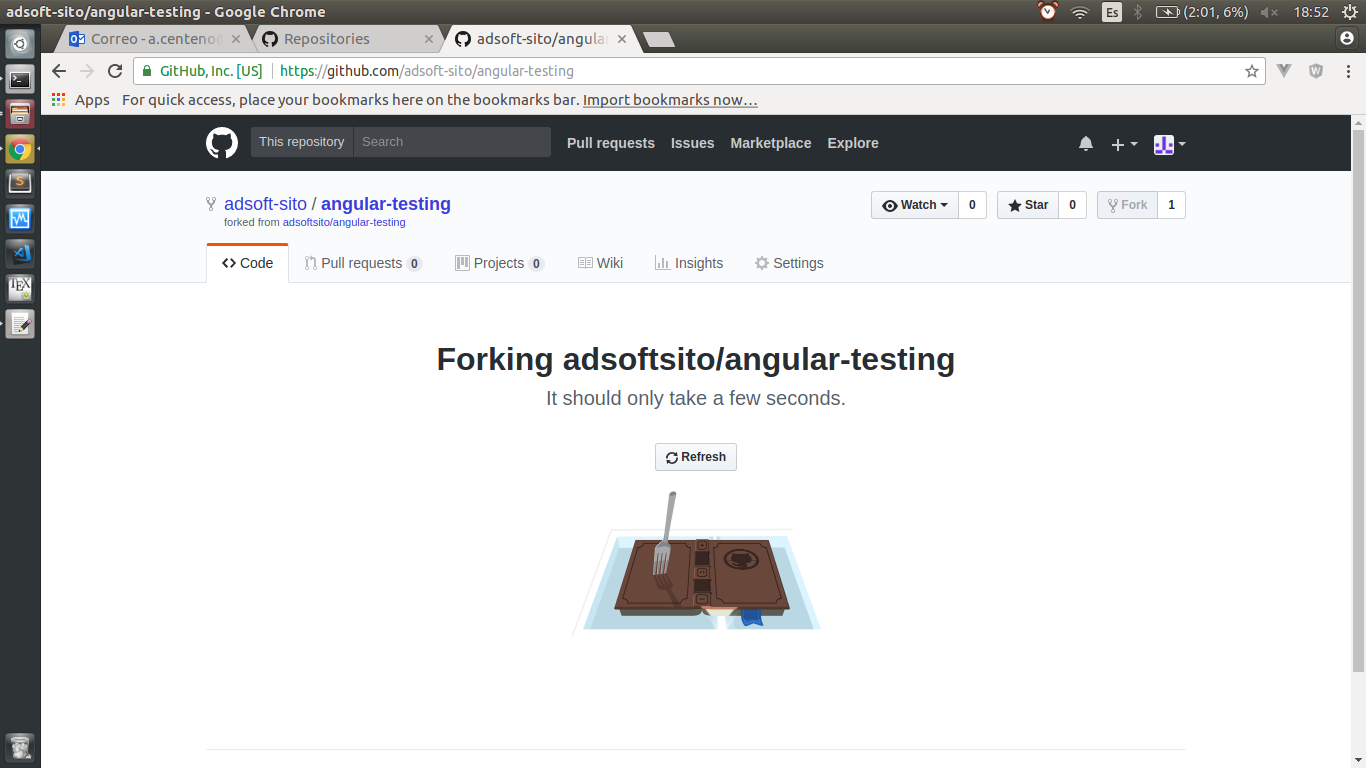
\includegraphics[width=0.9\textwidth]{forking.png}
\end{center}

\end{frame}

\begin{frame}\frametitle{} 

\begin{block}{clone your repo}
mkdir dev-testing \\
cd dev-testing	 \\
git clone -b develop https://github.com/your-own-repo/angular-testing.git \\
cd angular-testing \\
npm install \\
ng test   
\end{block}

\end{frame}


\begin{frame}\frametitle{} 

\begin{block}{compute branch}
git branch \\
git branch compute \\
git checkout compute \\
git merge develop compute \\
git branch 
\end{block}

\end{frame}


\begin{frame}\frametitle{} 

\begin{block}{create compute feature}
cd src/app \\
mkdir compute \\
cd compute
\end{block}

\begin{block}{nano compute.spec.ts}
\lstspec
\end{block}


\end{frame}




\begin{frame}\frametitle{} 


\begin{block}{nano compute.ts}
\lstts
\end{block}

\end{frame}


\begin{frame}\frametitle{} 


\begin{block}{push compute}
cd .. \\
cd .. \\
pwd  \\
git add src/app/compute \\
git commit -m "compute feature" \\
git push -u origin compute \\
\end{block}
\end{frame}


\begin{frame}\frametitle{} 

\begin{block}{Go to github}
\url{https://github.com/} \\

create a pull-request to develop branch in lider repo
\end{block}

\begin{center}
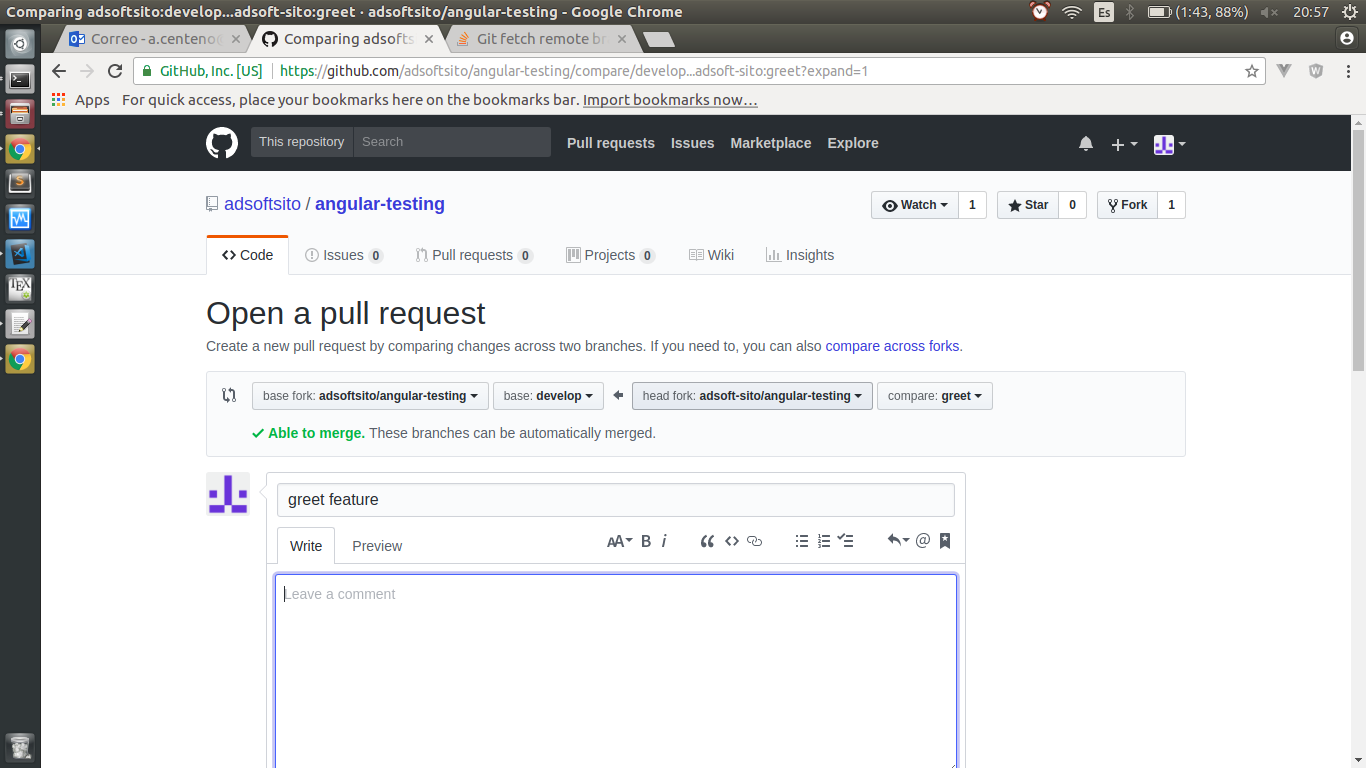
\includegraphics[width=0.9\textwidth]{pull-request.png}
\end{center}


\end{frame}

\end{document}
